\section{12.1 Wady metod bezpośrednich}

\begin{frame}{Wady metod bezpośrednich}
  \begin{block}{\textbf{Złożoność obliczeniowa} ${\sim}N^3$}
    \begin{itemize}
      \item{ $M=\frac{1}{3}n^3+n^2-\frac{1}{3}n$ ($\cdot$,$/$)}
      \item{ $D=\frac{1}{3}n^3+\frac{1}{2}n^2-\frac{5}{6}n$ ($+$)}
    \end{itemize}
    Np. $10^4$ punktów siatki przestrzennej (mesh points)
    \begin{itemize}
      \item{ na przykład 100 x 100   (2 -- D)}
      \item{metoda eliminacji Gaussa to $\sim (10^4)^3=10^{12}$ operacji}
      \item{jeśli 1 operacja trwa $\sim 10^{-8}$ s.}
      \item{to całość trwa $10^4$ czyli $\sim$ 3 godziny}
    \end{itemize}
  \end{block}
\end{frame}

\begin{frame}{}
  \begin{block}{\textbf{Zwykle}}
    \begin{itemize}
      \item{czas symulacji $\sim$ 1h,}
      \item{liczba kroków czasowych $\sim$ 1000,}
      \item{cały krok - to rozwiązywanie układu równań,}
      \item{1 operacja $\sim 10^{-8}$ s,}
      \item{liczba punktów siatki $\sim 10^4$ ($\equiv$ liczba równań)}
    \end{itemize}
  \end{block}
  \begin{block}{\textbf{Potrzebne są metody o znacznie mniejszej złożoności}}
   Metody takie powinny być oparte na własnościach równań różniczkowych cząstkowych (zwykle - źródła równań liniowych)
%   \begin{itemize}
  %    \item{liniowość,}
 %     \item{wymiar,}
  %    \item{możliwość separacji zmiennych,}
  %    \item{zakres zmian współczynników,}
  %    \item{kształt geometryczny obszaru,}
  %    \item{warunki brzegowe - postać.}
   % \end{itemize}
\end{block}
\end{frame}

\begin{frame}{Modelowe zadanie}
    Równanie Poissona - opisuje  niektóre procesy zachodzące w przyrodzie, np.
    \begin{itemize}
        \item potencjał pola grawitacyjnego 
        \item potencjał pola elektrostatycznego 
        \item rozkład temperatury wewnątrz ciała itp. 
     \end{itemize}

    \fbox{$\nabla^2
    \varphi(x,y)=-\rho(x,y)$}\\
    
   gdzie: $\varphi(x,y)$ - np. rozkład temperatury w 2D\\
   $\rho(x,y)$ -- funkcja rozkładu źródeł, zakładamy $\infty$ szybkość propagacji informacji\\

 $\nabla^2$ - operator Laplace'a, inaczej można zapisać to równanie:\\
  \fbox{
  $\frac{\partial^2 	\varphi(x,y)}{\partial x^2}+
  \frac {\partial^2 	\varphi(x,y)}{\partial y^2}=-\rho(x,y)$ }
  
\end{frame} 
\begin{frame}{Warunki brzegowe}
		
		Dla przykładowego równania:
		$$
		\frac{\partial^2 	\varphi(x,y)}{\partial x^2}+
  \frac {\partial^2	\varphi(x,y)}{\partial y^2}=-\rho(x,y) 
		$$
		Zakładamy przykładowe warunki brzegowe (np. na brzegach temperatura zawsze 0) :
		$$
		\varphi(0,y)=0, \varphi(n+1,y)=0,
		\varphi(x,0)=0, \varphi(x,n+1)=0
		$$
\end{frame}

\begin{frame}{Częste źródło układów równań Ax=B}
Metoda różnic skończonych\\
Cel: Przybliżenie pochodnych różnicami skończonymi
		Wprowadzamy siatkę:
		\begin{itemize}
			\item  $\varphi_{i,j} = \varphi(x_i, y_j),$ $i = 1,...,N,$ $j=1,...,M$
			\item $(x_i, y_i)$ - punkty siatki
			
			\item dla $i=0$, $i=N+1$, $j=0$, $j=M+1$ stosujemy warunki brzegowe \item zakładamy, że $h = x_{i+1}-x_i=y_{j+1}-y_j$ - odstępy między punktami
		\end{itemize}

		$$\frac{\partial \varphi_{i,j}}{\partial x} = \frac{\varphi_{i+1,j} - \varphi_{i-1,j}}{2h} + O(h^2)$$ \\
		$$\frac{\partial^2 \varphi_{i,j}}{\partial x^2} = \frac{\varphi_{i+1,j} - 2 \varphi_{i,j} + \varphi_{i-1,j}}{h^2} + O(h^2)$$
		Podobnie pochodne po $y$
	\end{frame}
%%%%%%%%%%%%%%%%

\begin{frame}{Przejście z równania różniczkowego na układ równań}
		Przybliżając pochodne różnicami skończonymi otrzymujemy:
		\begin{equation*}
		    \begin{split}
		    \frac{\varphi(x_{i+1},y_j) - 2 \varphi(x_i,y_j) + \varphi(x_{i-1}, y_j)}{h^2} +\\ \frac{\varphi(x_i,y_{j+1}) - 2 \varphi(x_i,y_j) + \varphi(x_{i},y_{j-1})}{h^2}=
		    -\rho(x_i,y_j) 
		\end{split}
		\end{equation*}
	Czyli:
		{\scriptsize
\begin{equation*}
		    \begin{split}
	 \frac{\varphi(x_{i},y_{j-1})  + \varphi(x_{i-1}, y_j)
	  - 4 \varphi(x_i,y_j)
	  +\varphi(x_{i+1},y_{j})
	 +\varphi(x_{i},y_{j+1})}{h^2} = -\rho(x_i,y_j) 
\end{split}
		\end{equation*}}

\end{frame}

%%%%%%%%%%%%%%%% 
\begin{frame}{Metoda roznic skonczonych}
  \begin{figure}
      \centering
      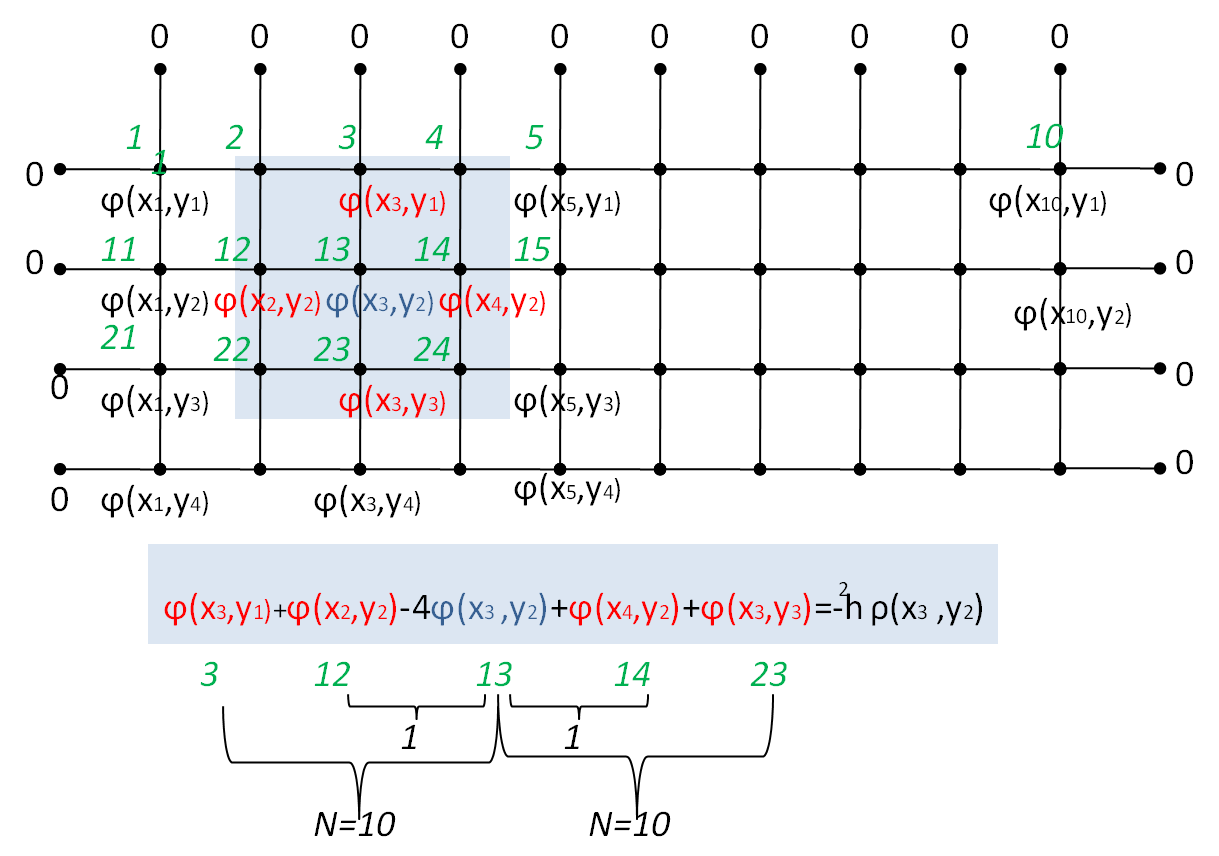
\includegraphics[width=\textwidth]{img/12/rozniczowe.png}
      \label{fig:my_label}
  \end{figure}  
\end{frame}
\begin{frame}{Metoda różnic skończonych - zapis macierzowy}
Wtedy równanie do rozwiązania wyglada tak:
	\begin{exampleblock}{Zapis macierzowy }
	{\scriptsize
	$$
	\begin{bmatrix}
	-4 & 1 &  &  & 1 &  & \\ 
	1&  -4 & 1 &  &  &1  & \\ 
	& 1 &  -4& 1 &  &  &1 \\ 
	1&  &  ...& &  &  & \\ 
	& 1 &  &  1 & -4 & 1 & \\ 
	&  & 1 &  & 1 &  -4 &
	\end{bmatrix}		
	\begin{bmatrix}
	\varphi(x_1,y_1) \\
	\varphi(x_2,y_1) \\
	\varphi(x_3,y_1) \\
	...\\
	\varphi(x_n,y_{n-1})\\
	\varphi(x_n, y_{n})\\
	\end{bmatrix}		
	= 		
	\begin{bmatrix} 
	-h^2\rho(x_1,y_1)  \\
	-h^2\rho(x_2,y_1)\\
	-h^2\rho(x_3,y_1)\\
	... \\
	-h^2\rho(x_n,y_{n-1})\\
	-h^2\rho(x_n, y_{n})\\
	\end{bmatrix}
	$$}
	\end{exampleblock}
\end{frame}
\begin{frame}{}
  \textbf{Metody bezpośrednie zaburzają strukturę macierzy rzadkich}
  \newline Przykład: niewiadomą jest  wielkość w każdym punkcie siatki (lewy rysunek), która zależy od swoich najbliższych sąsiadów.\\
  Prawy rysunek pokazuje odpowiadające  równanie liniowe. %2 - D $\rightarrow$ operator pięciopunktowy
  \begin{figure}
    \centering
    \includegraphics[height=0.75\textheight, width=1.1\textwidth]{img/12/iteracja1}
  \end{figure}
\end{frame}

\begin{frame}{}
  \begin{block}{\textbf{Metody bezpośrednie zaburzają strukturę macierzy rzadkich}}
    \begin{itemize}
      \item macierz wstęgowa ma {$\sim 5 \cdot N^2$ współczynników $\neq$ 0}
      \item{ale: po zastosowaniu metody eliminacji Gaussa znikają zera z wstęg (tam gdzie (*) na rysunku)
      \newline  $\rightarrow$ trzeba wtedy pamiętać $2 \cdot N^3$ współczynników}
      % na pózniej
      %\item{Macierz wstęgowa: $m_{ij}=0$ dla $|i-j|>k$}
     % \item W metodach polegających na mnożeniu $A \cdot x^{(t)}$ w kroku t zamiast $n^2 \rightarrow k \cdot n$ mnożeń $\Rightarrow$ wtedy łatwo o:
     % \begin{center}
     % $s \cdot k \cdot n<n^3$
     % \end{center}
    %  \item gdzie s - liczba kroków, a $n^3$ - złożoność metod bezpośrednich.
    \end{itemize}
  \end{block}
\end{frame}

%%%%%%%%%%%%%%%%
